\section{Example}

\begin{figure}[H]
    \begin{center} 
        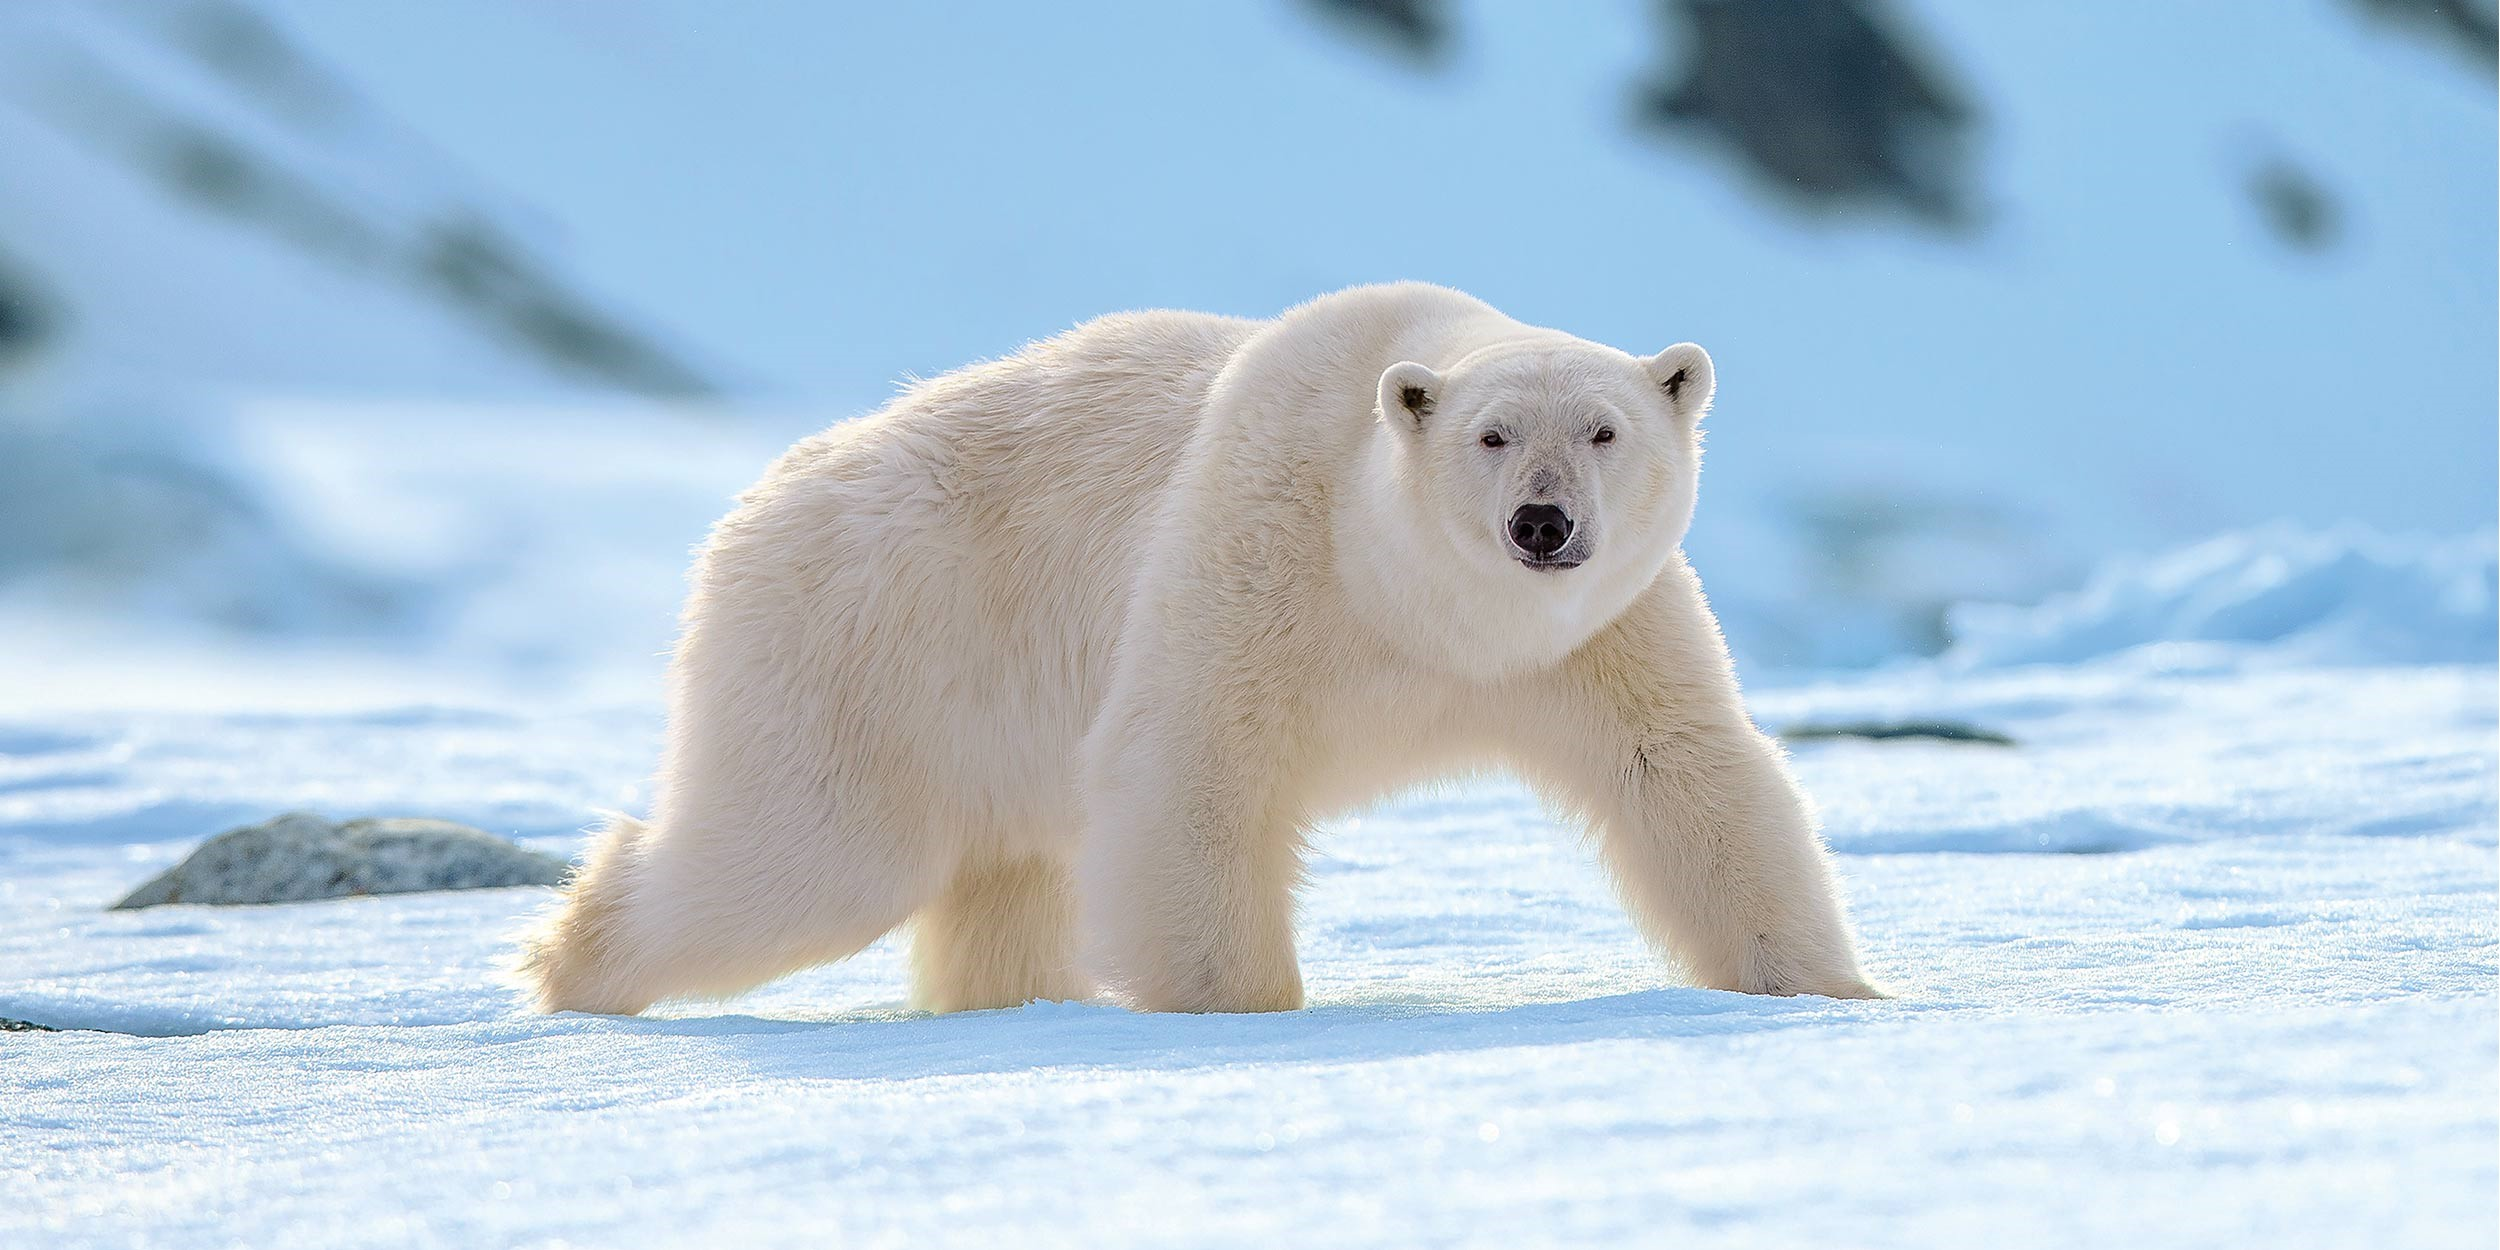
\includegraphics[width=0.8\textwidth]{example}
        \caption{Example Image}
        \label{fig:example}
    \end{center}
\end{figure}

\cite[vgl. dazu][]{example-book}

This Picture (\ref{fig:example}) is awesome

\cite[vgl. dazu][]{example-online}

\newpage

\section{Requirements}

\srequirement{should}
lala und lulu

\corequirement{could}
lala und lulu

\morequirement{could}
lala und lulu

\wrequirement{could}
lala und lulu

\section{Programming}

\begin{lstlisting}[language=Bash]
#!/bin/bash

echo "Hello World"
\end{lstlisting}

\begin{lstlisting}[language=Python]
# same in python

print("Hello World")
\end{lstlisting}

\begin{verbatim}
$ sudo apt-get update
$ sudo apt-get install python
\end{verbatim}
